%% -------------------------------------------------------------- %%
% 								   %
%                     FICHES TECHNIQUES LATEX       	           %
%                      Ecole Centrale de Lyon			   %
%             Template LaTeX : Copyright Damien Douteaux           %
%                       Décembre 2016 - Lyon                       %
% 								   %
%% -------------------------------------------------------------- %%


%% -------------------------------------------------------------- %%
%								   %
%                         Type du document			   %
%								   %
%% -------------------------------------------------------------- %%

\documentclass[11pt,a4paper]{article}

%% -------------------------------------------------------------- %%
%								   %
%            Importation des fichiers de configuration             %
%								   %
%% -------------------------------------------------------------- %%

%
% 1 - Fichier d'import des packages
%
%% Global libraries
\usepackage[
        twoside,
	top=27mm,
	bottom=27mm,
	inner=20mm,
	outer=20mm,
	ignorehead,
	ignorefoot,
	includemp,
	marginparwidth=52mm,
	marginparsep=8mm,
	headsep=7mm,
	footskip=14mm,
        headheight=15pt]{geometry}
\usepackage[french]{babel} % language type annotations

%% Libraries for graphics and colours
\usepackage{tikz} % for drawing
\usepackage{graphicx} % improve include graphics
\usepackage{lipsum} % for testing
\usepackage[most]{tcolorbox} % to have fill paterns for TikZ
\usepackage{changepage} % for adjustwidth command
\usepackage{xcolor} % to have access to every immaginable color
\usepackage{colortbl}
\usepackage{amsmath} % mathematics package
\usepackage{amssymb} % mathematics symbols
\usepackage[explicit,pagestyles]{titlesec} % redefine titles style
\usepackage{mdframed} % permet de couper du texte entre plusieurs pages
\usepackage{framed}
\usepackage{titletoc} % redefine toc
\usepackage{etoolbox} % ?? (used to redefine toc)
\usepackage{stmaryrd}
\usepackage{ifthen} % use to make if then conditions
\usepackage{tikzscale} % in order to scale TikZ pictures
\usepackage{multicol}
\usepackage{capt-of}
\usepackage{xspace}
\usepackage{array}
\usepackage[normalem]{ulem}
\usepackage{url}
\usepackage{subcaption}
\usepackage{cite}
\usepackage{pdftexcmds} % Comparaison de string dans switch case
\usepackage{fancyhdr}
\usepackage{marginnote}
\usepackage{calc}

%% Other libraries
\usepackage{eurosym} % in order to have € symbol
\usepackage{notoccite} % helps for quotations
\usepackage{float} % helps to place figures
\usepackage[unicode]{hyperref} % in order to make hyperref links inside doc
\usepackage{setspace} % in order to help adding space in the document
\usepackage{longtable} % in order to have multipage tables
\usepackage{multirow} % in order to use multirow in a table
\usepackage{pifont} % in order to have checkmarks and crosses
\usepackage{booktabs} % to have predefined tab rules
\usepackage{rotating} % to have rotating boxes
\usepackage{tkz-tab}
\usepackage{mathrsfs}

%% TikZ libraries needed to compute
\usetikzlibrary{fit} 
\usetikzlibrary{graphs} % package for graphics representation
\usetikzlibrary{positioning} % possitionning inside TikZ picture
\usetikzlibrary{arrows} % beautiful arrows with TikZ
\usetikzlibrary{calc} % enable computation of values insidecture
\usetikzlibrary{decorations} % decoration for TikZ picture
%%% Local Variables:
%%% mode: plain-tex
%%% TeX-master: "../Template"
%%% End:


%
% 2 - Fichier de configuration utilisateur
%
\definecolor{themeColor}{RGB}{0,107,47}
\definecolor{vertforet}{RGB}{20,83,20}
\definecolor{vvertforet}{RGB}{0,107,47}
\definecolor{bordeau}{RGB}{199,16,26}
\definecolor{gris}{RGB}{195,195,195}
\definecolor{bluenight}{RGB}{0,82,148}
\definecolor{bluesword}{RGB}{0,82,148}
\definecolor{violet}{RGB}{112,4,98}
\definecolor{amber}{RGB}{255,110,0}
\definecolor{mygray}{RGB}{125,125,125}

\newcommand{\currentColor}{themeColor}
\newcommand{\headersColor}{themeColor}
%\def \currentColor {themeColor}
\newcommand\thColor[1]{\textcolor{themeColor}{#1}}
\newcommand\curColor[1]{\textcolor{\currentColor}{#1}}
\newcommand\headColor[1]{\textcolor{\headersColor}{#1}}
\newcommand\wiColor[1]{\textcolor{white}{#1}}

%%% Local Variables:
%%% mode: plain-tex
%%% TeX-master: "../Master"
%%% End:

%%---------------------------------------------------------------%%
%                                                                 %
%   Fichier de toutes les configurations basiques utilisateurs    %
%                                                                 %
%%---------------------------------------------------------------%%

%
% 1 - Positionnement des TOC - LOF - LOT dans le document
%
\newcommand\whereTOC{beginning}          % Parmis beginning - end
\newcommand\whereLOF{end}                % Parmis beginning - end
\newcommand\whereLOT{end}                % Parmis beginning - end
\newcommand\TOCLOFTNumStyle{Roman}       % Parmis Roman - roman - Arabic - arabic
\newcommand\LOFLOTSeparator{\vfill}      % Séparateur après une LOF ou LOT
\newcommand\TOCSeparator{\newpage}       % Séparateur après un TOC
\newcommand\inclureTOC{true}             % Mettre la TOC (true) ou pas (false)
\newcommand\inclureLOF{false}            % Mettre la LOF (true) ou pas (false)
\newcommand\inclureLOT{false}            % Mettre la LOT (true) ou pas (false)

%
% 2 - Fichiers à inclure
%
\newcommand\inclureIntroduction{false}   % Mettre l'introduction (true) ou pas (false)    -> Position imposée
\newcommand\inclureConclusion{false}     % Mettre la conclusion (true) ou pas (false)     -> Position imposée
\newcommand\inclureRemerciements{false}  % Mettre les remerciements (true) ou pas (false)
\newcommand\inclureResume{false}         % Mettre le résumé (true) ou pas (false)
\newcommand\inclureAbstract{false}       % Mettre le résumé anglais (true) ou pas (false)
\newcommand\inclureReferences{false}     % Mettre les références (true) ou pas (false)
\newcommand\whereResume{beginning}       % Parmis beginning - end
\newcommand\whereRemerciements{beginning}% Parmis beginning - end
\newcommand\whereReferences{end}         % Parmis beginning - end

%
% 3 - Informations pour en-têtes et pieds de page
%
\newcommand\footerRight{\textbf{Année 2017}   }                    % À gauche séparation du footer
\newcommand\footerLeft{\textbf{\thepage}}                          % À droite séparation du footer
\newcommand\headerText{\textbf{Principe et applications de XGBoost}}   % Texte de l'en-tête
\newcommand\headerLogo{logo}                                       % Logo de l'en-tête (optionnel)

%
% 4 - Page de titre à charger
%
\newcommand\titlePage{picture}                                     % Voir les noms dans conf/Pages_titre/

%
% 5 - Le type de sections désiré
%

% 5.1 - Aspect d'une partie
\newcommand\partFormat{page}
\newcommand\partModele{default}
% 5.2 - Aspect d'une section
\newcommand\sectionFormat{default}
\newcommand\sectionNumber{arabic}
\newcommand\sectionNumberStyle{textbfc}
\newcommand\sectionSeparator{~~$\bullet$~~}
\newcommand\sectionSeparatorStyle{thColor}
\newcommand\sectionTextStyle{textbfc}
% 5.3 - Aspect d'une sous-section
\newcommand\subsectionFormat{default}
\newcommand\subsectionNumber{arabic}
\newcommand\subsectionNumberStyle{thColor}
\newcommand\subsectionSeparator{}
\newcommand\subsectionSeparatorStyle{}
\newcommand\subsectionTextStyle{thColor}
% 5.4 - Aspect d'une sous-sous-section
\newcommand\subsubsectionFormat{default}
\newcommand\subsubsectionNumber{arabic}
\newcommand\subsubsectionNumberStyle{thColor}
\newcommand\subsubsectionSeparator{}
\newcommand\subsubsectionSeparatorStyle{}
\newcommand\subsubsectionTextStyle{textit}
% 5.5 - Aspect d'un paragraphe
\newcommand\paragrapheFormat{default}
\newcommand\paragrapheNumber{none}        % Pas de numérotation (none), autrement {Roman ; roman ; arabic ; Arabic}
\newcommand\paragrapheNumberStyle{}
\newcommand\paragrapheSeparator{}
\newcommand\paragrapheSeparatorStyle{}
\newcommand\paragrapheTextStyle{}
% 5.6 - Aspect d'un sous-paragraphe
\newcommand\subparagrapheFormat{default}
\newcommand\subparagrapheNumber{none}     % Pas de numérotation (none), autrement {Roman ; roman ; arabic ; Arabic}
\newcommand\subparagrapheNumberStyle{}
\newcommand\subparagrapheSeparator{}
\newcommand\subparagrapheSeparatorStyle{}
\newcommand\subparagrapheTextStyle{textic}
% 5.7 - Aspect de la page d'annexe
\newcommand\annexeModele{default}         % Aucune (none) ou voir dans conf/Pages_annexes/

%
% 6 - Pour les sections avec images, configuration des images
%
\newcommand\imageSectionI{default1}
\newcommand\imageSectionII{default2}
\newcommand\imageSectionIII{default3}
\newcommand\imageSectionIV{default4}
\newcommand\imageSectionV{default5}
%%---------------------------------------------------------------%%
%                                                                 %
%       !!! NE PAS CHANGER SAUF SI ON SAÎT CE QU'ON FAIT !!!      %
%      Inclusions automatiques en fonction des configurations     %
%                                                                 %
%%---------------------------------------------------------------%%

% 1 - La page de garde
\input{conf/Pages_garde/page_garde__\titlePage}       % Charger les configurations de cette page titre

% 2 - La page d'aspect de partie
\input{conf/Pages_parties/part__\partModele}    % Charger les configurations du bon modèle de page pour les parties

% 3 - La page d'aspect des annexes
\input{conf/Pages_annexes/annexe__\annexeModele}  % Charger les configurations du bon modèle de page pour les parties

%
% 3 - Fichier de définition des styles
%
%
% Méthode pour l'inclusion automatique de fichier/élément à l'endroit désiré
% Params :
%     1 - Elément à inclure
%     2 - Configuration pour le choix (\whereXXX)
%     3 - Endroit à tester
%     4 - S'il y a possibilité de ne pas inclure l'élément
%
\makeatletter
\newcommand{\whereIncludeFile}[4]{
  \ifnum\pdf@strcmp{#4}{true}=0
  \ifnum\pdf@strcmp{#2}{#3}=0
  #1
  \fi\fi
}
\makeatother

\newcommand{\includeTOC}[1]{
  \whereIncludeFile{\clearpage\tableofcontents\TOCSeparator}{\whereTOC}{#1}{\inclureTOC}
}

\newcommand{\includeLOF}[1]{
  \whereIncludeFile{\listoffigures\LOFLOTSeparator}{\whereLOF}{#1}{\inclureLOF}
}

\newcommand{\includeLOT}[1]{
  \whereIncludeFile{\listoftables\LOFLOTSeparator}{\whereLOT}{#1}{\inclureLOT}
}

\newcommand{\includeResume}[1]{
  \whereIncludeFile{\nnsection{Résumé}
Ceci est le résumé du document

\begin{figure}[ht]
  \caption{Une figure magnifique}
  \label{fig:mafig}
\end{figure}

\begin{table}[ht]
  \caption{Un tableau vital pour la suite}
  \label{tab:vital}
\end{table}


%%% Local Variables:
%%% mode: latex
%%% TeX-master: "../../Template"
%%% End:
}{\whereResume}{#1}{\inclureResume}
}

\newcommand{\includeAbstract}[1]{
  \whereIncludeFile{\input{text/Pages_gnl/abstract.tex}}{\whereResume}{#1}{\inclureAbstract}
}

\newcommand{\includeRemerciements}[1]{
  \whereIncludeFile{\input{text/Pages_gnl/remerciements.tex}}{\whereRemerciements}{#1}{\inclureRemerciements}
}

\newcommand{\includeIntroduction}{
  \whereIncludeFile{\nnsection{Introduction}
\label{sec:introduction}
L'introduction du document

%%% Local Variables:
%%% mode: latex
%%% TeX-master: "../../Rapport_RO_BE1"
%%% End:
}{beginning}{beginning}{\inclureIntroduction}
}

\newcommand{\includeConclusion}{
  \whereIncludeFile{\nnsection{Conclusion}

%%% Local Variables:
%%% mode: latex
%%% TeX-master: "../../Rapport_dreches"
%%% End:
}{beginning}{beginning}{\inclureConclusion}
}

%
% Afficher un argument si l'autre est non vide
% Params :
%     1 - Texte à afficher
%     2 - Valeur de contrôle
%
%\newcommand{\printIfNotZero}[2]{
%  \ifnum#2=0
%  \else
%  #1
%  \fi
%}
\newcommand{\printIfNotZero}[2]{%
  \ifthenelse{#2=0}{}{#1}%
}

%%% Local Variables:
%%% mode: latex
%%% TeX-master: "../Template"
%%% End:

%
% Applique un formatage sur le texte fourni
% Params :
%     1 - Le format demandé
%     2 - Le texte à mettre en forme
%
\makeatletter
\newcommand{\applyFormat}[2]{%
  \ifnum\pdf@strcmp{#1}{textbi}=0%
  \textbi{#2}%
  \else\ifnum\pdf@strcmp{#1}{textbf}=0%
  \textbf{#2}%
  \else\ifnum\pdf@strcmp{#1}{textit}=0%
  \textit{#2}%
  \else\ifnum\pdf@strcmp{#1}{textsc}=0%
  \textsc{#2}%
  \else\ifnum\pdf@strcmp{#1}{textbic}=0%
  \textbic{#2}%
  \else\ifnum\pdf@strcmp{#1}{textbfc}=0%
  \textbfc{#2}%
  \else\ifnum\pdf@strcmp{#1}{textic}=0%
  \textic{#2}%
  \else\ifnum\pdf@strcmp{#1}{textscic}=0%
  \textbic{#2}%
  \else\ifnum\pdf@strcmp{#1}{textscc}=0%
  \textscc{#2}%
  \else\ifnum\pdf@strcmp{#1}{thColor}=0%
  \thColor{#2}%
  \fi\fi\fi\fi\fi\fi\fi\fi\fi\fi%
}
\makeatother

\newcommand\textbi[1]{%
  \textbf{\textit{#1}}%
}

\newcommand\textbic[1]{%
  \textbf{\textit{\thColor{#1}}}%
}

\newcommand\textbfc[1]{%
  \textbf{\thColor{#1}}%
}

\newcommand\textscic[1]{%
  \textsc{\textit{\thColor{#1}}}%
}

\newcommand\textscc[1]{%
  \textsc{\thColor{#1}}%
}

\newcommand\textic[1]{%
  \textit{\thColor{#1}}%
}
  

%%% Local Variables:
%%% mode: latex
%%% TeX-master: "../Template"
%%% End:

% Some pre-defined TikZstyles
\tikzset{
	sectionleft/.style={text height=1.5ex,text depth=0ex,color=\headersColor},
	drawrect/.style={draw, rectangle, fill=#1},
	footers/.style={draw, rectangle, minimum width=21cm, minimum height = 0.5cm, color=#1, fill=#1},
	headers/.style={draw, rectangle, minimum width=21cm, minimum height = 0.5cm, color=#1, fill=#1},
	headers/.default=\headersColor,
	footers/.default=\headersColor,
	drawrect/.default=\headersColor,
    rectangle with rounded corners north west/.initial=4pt,
    rectangle with rounded corners south west/.initial=4pt,
    rectangle with rounded corners north east/.initial=4pt,
    rectangle with rounded corners south east/.initial=4pt
}

\pgfdeclarelayer{background}
\pgfdeclarelayer{foreground}
\pgfsetlayers{background,main,foreground}

\makeatletter
\pgfdeclareshape{rectangle with rounded corners}{
  \inheritsavedanchors[from=rectangle] % this is nearly a rectangle
  \inheritanchorborder[from=rectangle]
  \inheritanchor[from=rectangle]{center}
  \inheritanchor[from=rectangle]{north}
  \inheritanchor[from=rectangle]{south}
  \inheritanchor[from=rectangle]{west}
  \inheritanchor[from=rectangle]{east}
  \inheritanchor[from=rectangle]{north east}
  \inheritanchor[from=rectangle]{south east}
  \inheritanchor[from=rectangle]{north west}
  \inheritanchor[from=rectangle]{south west}
  \backgroundpath{% this is new
    % store lower right in xa/ya and upper right in xb/yb
    \southwest \pgf@xa=\pgf@x \pgf@ya=\pgf@y
    \northeast \pgf@xb=\pgf@x \pgf@yb=\pgf@y
    % construct main path
    \pgfkeysgetvalue{/tikz/rectangle with rounded corners north west}{\pgf@rectc}
    \pgfsetcornersarced{\pgfpoint{\pgf@rectc}{\pgf@rectc}}
    \pgfpathmoveto{\pgfpoint{\pgf@xa}{\pgf@ya}}
    \pgfpathlineto{\pgfpoint{\pgf@xa}{\pgf@yb}}
    \pgfkeysgetvalue{/tikz/rectangle with rounded corners north east}{\pgf@rectc}
    \pgfsetcornersarced{\pgfpoint{\pgf@rectc}{\pgf@rectc}}
    \pgfpathlineto{\pgfpoint{\pgf@xb}{\pgf@yb}}
    \pgfkeysgetvalue{/tikz/rectangle with rounded corners south east}{\pgf@rectc}
    \pgfsetcornersarced{\pgfpoint{\pgf@rectc}{\pgf@rectc}}
    \pgfpathlineto{\pgfpoint{\pgf@xb}{\pgf@ya}}
    \pgfkeysgetvalue{/tikz/rectangle with rounded corners south west}{\pgf@rectc}
    \pgfsetcornersarced{\pgfpoint{\pgf@rectc}{\pgf@rectc}}
    \pgfpathclose
 }
}
\makeatother

%%% Local Variables:
%%% mode: plain-tex
%%% TeX-master: "../Master"
%%% End:

%%  boxing (general code)
\newcommand\generalencadrement[5]{\renewcommand{\currentColor}{#3}\vspace{0.3cm}\noindent\tikz{[line width=1]
\node (contentnode) [draw, color=#3, fill=#4, text=black, rectangle, inner sep = 15, outer sep = 0, rounded corners = 2mm, minimum width=\linewidth-1, text width=\linewidth-31,align=justify, right] at (0,0) {\newline #2};
\node [draw,rectangle,inner sep = 3,outer sep = 3,rounded corners = 1mm, fill opacity=1, above, color=#3, fill=#5, text =black, right]  at ([xshift=15]contentnode.north west) {\hspace{0.1cm}#1 \hspace{0.1cm}};
}\par\vspace{0.3cm}\renewcommand{\currentColor}{themeColor}}

\newcommand\customgeneralencadrement[5]{\vspace{.15cm}\begin{tcolorbox}[breakable, title={#1}, attach boxed title to top left= {xshift=10mm,yshift=-3mm}, boxed title style={boxrule=.8pt}, colframe=#3, colback=#5, coltitle=black, colbacktitle=#4, boxrule=.8pt]
\vspace{.3cm}
#2
\end{tcolorbox}}

%% Several types of useful boxes (using previous source code)
\newcommand\remarqueencadr[1]{\par\generalencadrement{ Remark }{ #1 }{vertforet}{white}{white}}
\newcommand\attentionencadr[1]{\par\generalencadrement{ Beware }{ #1 }{bordeau}{white}{white}}
\newcommand\informationencadr[1]{\par\generalencadrement{ Information }{ #1 }{orange}{white}{white}}
\newcommand\paragrapheencadr[2]{\par\generalencadrement{ #1 }{ #2 }{themeColor}{white}{white}}

\newcommand\remarqueencadrfond[1]{\par\generalencadrement{ Remark }{ #1 }{vertforet}{vertforet!50}{white}}
\newcommand\attentionencadrfond[1]{\par\generalencadrement{ Beware }{ #1 }{bordeau}{bordeau!50}{white}}
\newcommand\informationencadrfond[1]{\par\generalencadrement{ Information }{ #1 }{orange}{orange!50}{white}}
\newcommand\paragrapheencadrfond[2]{\par\generalencadrement{ #1 }{ #2 }{themeColor}{themeColor!50}{white}}

\newcommand\remarqueencadrfondd[1]{\par\generalencadrement{ Remark }{ #1 }{vertforet}{vertforet!5}{vertforet!50}}
\newcommand\attentionencadrfondd[1]{\par\generalencadrement{ Beware }{ #1 }{bordeau}{bordeau!5}{bordeau!50}}
\newcommand\informationencadrfondd[1]{\par\generalencadrement{ Information }{ #1 }{orange}{orange!5}{orange!50}}
\newcommand\paragrapheencadrfondd[2]{\par\generalencadrement{ #1 }{ #2 }{themeColor}{themeColor!5}{themeColor!50}}

\newcommand\mathdefinition[2]{\par\generalencadrement{ Definition --- #1 }{ #2 }{bluenight}{white}{white}}
\newcommand\mathdefinitionvoid[1]{\par\generalencadrement{ Definition }{ #1 }{bluenight}{white}{white}}
\newcommand\maththeoreme[2]{\par\generalencadrement{ Theorem --- #1 }{ #2 }{vertforet}{white}{white}}
\newcommand\maththeoremevoid[1]{\par\generalencadrement{ Theorem }{ #1 }{vertforet}{white}{white}}
\newcommand\mathpropriete[2]{\par\generalencadrement{ Propriety --- #1 }{ #2 }{orange}{white}{white}}
\newcommand\mathproprietevoid[1]{\par\generalencadrement{ Propriété }{ #1 }{orange}{white}{white}}
\newcommand\mathcasparticulier[2]{\par\generalencadrement{ Particular case --- #1 }{ #2 }{violet}{white}{white}}
\newcommand\mathcasparticuliervoid[1]{\par\generalencadrement{ Particular case }{ #1 }{violet}{white}{white}}
\newcommand\mathmethode[2]{\par\generalencadrement{ Method --- #1 }{ #2 }{bordeau}{white}{white}}
\newcommand\mathexercice[2]{\par\generalencadrement{ Exercise #1 }{ #2 }{bluenight}{white}{white}}
\newcommand\mathenonce[1]{\par\generalencadrement{ Problem statement }{ #1 }{bluenight}{white}{white}}
\newcommand\mathproposition[2]{\par\generalencadrement{ Proposition --- #1 }{ #2 }{orange}{white}{white}}
\newcommand\mathpropositionvoid[1]{\par\generalencadrement{ Proposition }{ #1 }{orange}{white}{white}}

%% Boxes to enhanced results
\newcommand{\result}[1]{\tresult{$\displaystyle{#1}$}}
\newcommand{\tresult}[1]{\colorbox{themeColor!30}{#1}}

%%% Local Variables:
%%% mode: latex
%%% TeX-master: "../Master"
%%% End:

%% Rededefining table of contents
\addto\captionsfrench{ % French stands for the used language
  \renewcommand{\contentsname}{Table des matières}%
  \renewcommand{\listfigurename}{Liste des figures}%
  \renewcommand{\listtablename}{Liste des tables}%
}

\makeatletter
%% Style des sections dans la TOC
\titlecontents{section}
[0em]
{\vspace{.25cm}\color{themeColor}\Large}
{\rule[-2pt]{.2cm}{\f@size pt}~~\contentslabel{}\quad\raisebox{1pt}{$\bullet$}\enspace}
{\rule[-2pt]{.2cm}{\f@size pt}~~}
{\titlerule*[0.7em]{.}\rmfamily\upshape\contentspage}
[]

%% Style des sous-sections dans la TOC
\titlecontents{subsection}
[2em]
{}
{\hspace*{4em}\thColor{\contentslabel{2em}}}
{}
{\titlerule*[0.7em]{.}\rmfamily\upshape\contentspage}
[]

%% Style des sous-sections dans la TOC
\titlecontents{subsubsection}
[4em]
{}
{\hspace*{6em}\textbf{\contentslabel{3em}}}
{}
{\titlerule*[0.7em]{.}\rmfamily\upshape\contentspage}
[]


%% Styles des sous-sections dans la mini-TOC
\titlecontents{psubsection}
[0em] % distance from left margin
{\Large} % above (global formatting of entry)
{\hspace*{2em}\thColor{\contentslabel{2em}}} % before w/label (label = ``2.6'')
{} % before w/o label
{\titlerule*[0.7em]{.}\rmfamily\upshape\contentspage} % filler + page (leaders and page num)
[] % after
\makeatother
  
%% Intermidiate table of contents
\newcommand\PartialToC{
  \begin{adjustwidth}{2cm}{2cm}
    \startcontents[sections]%
    \noindent\begin{mdframed}[backgroundcolor=white, hidealllines=true]
      \printcontents[sections]{p}{1}{}
    \end{mdframed}
  \end{adjustwidth}
}

%%% Local Variables:
%%% mode: latex
%%% TeX-master: "../Rapport_dreches"
%%% End:

%% Easier way to include graphics
%% Caption package
\usepackage{caption}
\DeclareCaptionLabelSeparator{bullet}{~\headColor{$\bullet$}~}
\captionsetup{labelfont={bf,color=\headersColor},labelsep=bullet}

\newcommand{\figurePerso}[4]{\begin{figure}[!ht]\centering\includegraphics[#1]{#2}\caption{#3}\label{#4}\end{figure}}
\newcommand{\figurePersoTikz}[3]{\begin{figure}[h]\makebox[\textwidth][c]{\input{#1}}\caption{#2}\label{#3}\end{figure}}
\newcommand{\figurePersoTikzz}[3]{\begingroup\centering\input{#1}\captionof{figure}{#2}\label{#3}\endgroup}
\newcommand{\figurePersoTikzSansCaption}[1]{\begingroup\centering\input{#1}\endgroup}
%% Defining our itemize bullet
\newcommand\mybullet{\tikz{\draw [color=\currentColor, fill=\currentColor] (0,0) circle [radius=.03cm]; \draw [color=\currentColor,thick] (0,0) circle [radius=0.1cm];}}

\newcommand\itemperso[1]{\item[\mybullet]~\textit{\textcolor{\currentColor}{#1}}\ifthenelse{\equal{#1}{}}{}{\hspace{0.5cm}}}

\newcommand{\tabitem}{~~\llap{\mybullet}~~}

\newcommand\subitemperso[1]{\item[\textcolor{\currentColor}{$\triangleright$}] \textit{\textcolor{\currentColor}{#1}}\ifthenelse{\equal{#1}{}}{}{\hspace{0.2cm}}}

\newcommand\subsubitemperso[1]{\item[\textcolor{\currentColor}{$\star$}] \textit{\textcolor{\currentColor}{#1}}\ifthenelse{\equal{#1}{}}{}{\hspace{0.2cm}}}

%% New items for school work questions
\newcommand\exquestion[1]{\vspace{.1cm}\item[\mybullet] \textcolor{\currentColor}{#1}\ifthenelse{\equal{#1}{}}{}{\hspace{0.5cm}}}

\newcommand\exsubquestion[1]{\item[\textcolor{\currentColor}{$\triangleright$}] \textcolor{\currentColor}{#1}\ifthenelse{\equal{#1}{}}{}{\hspace{0.2cm}}}

\newcommand\exsubsubquestion[1]{\item[\textcolor{\currentColor}{$\star$}] \textcolor{\currentColor}{#1}\ifthenelse{\equal{#1}{}}{}{\hspace{0.2cm}}}

%% Commands to define tick, cross and neutral mark
\newcommand{\cmark}{\textcolor{vertforet}{\ding{51}}}%
\newcommand{\xmark}{\textcolor{bordeau}{\ding{55}}}%
\newcommand{\neutral}{\textcolor{gray}{\ding{70}}}%
\newcommand\testStatus[1]{\ifthenelse{\equal{#1}{OK}}{\cmark}{\ifthenelse{\equal{#1}{NSP}}{\neutral}{\xmark}}}

\newcommand\itemtest[3]{\itemperso{}\begin{minipage}[t]{\dimexpr\linewidth-.5cm\relax}%
	\textit{\textcolor{themeColor}{#1}}\ifthenelse{\equal{#1}{}}{}{\hspace{0.5cm}}#2\end{minipage}%
	\hspace{\fill}\testStatus{#3}}
\newcommand\subitemtest[3]{\subitemperso{}\begin{minipage}[t]{\dimexpr\linewidth-.5cm\relax}%
	\textit{\textcolor{themeColor}{#1}}\ifthenelse{\equal{#1}{}}{}{\hspace{0.5cm}}#2\end{minipage}%
	\hspace{\fill}\testStatus{#3}}
\newcommand\subsubitemtest[3]{\subsubitemperso{}\begin{minipage}[t]{\dimexpr\linewidth-.5cm\relax}
	\textit{\textcolor{themeColor}{#1}}\ifthenelse{\equal{#1}{}}{}{\hspace{0.5cm}}#2\end{minipage}%
	\hspace{\fill}\testStatus{#3}}

\newcommand\itemtestdouble[4]{\itemperso{}\begin{minipage}[t]{\dimexpr\linewidth-1cm\relax}%
	\textit{\textcolor{themeColor}{#1}}\ifthenelse{\equal{#1}{}}{}{\hspace{0.5cm}}#2\end{minipage}%
	\hspace{\fill}\testStatus{#3}\hspace{\fill}\testStatus{#4}}
\newcommand\subitemtestdouble[4]{\subitemperso{}\begin{minipage}[t]{\dimexpr\linewidth-1cm\relax}%
	\textit{\textcolor{themeColor}{#1}}\ifthenelse{\equal{#1}{}}{}{\hspace{0.5cm}}#2\end{minipage}%
	\hspace{\fill}\testStatus{#3}\hspace{\fill}\testStatus{#4}}
\newcommand\subsubitemtestdouble[4]{\subsubitemperso{}\begin{minipage}[t]{\dimexpr\linewidth-1cm\relax}
	\textit{\textcolor{themeColor}{#1}}\ifthenelse{\equal{#1}{}}{}{\hspace{0.5cm}}#2\end{minipage}%
	\hspace{\fill}\testStatus{#3}\hspace{\fill}\testStatus{#4}}

\newcommand\itemtesttriple[5]{\itemperso{}\begin{minipage}[t]{\dimexpr\linewidth-1.5cm\relax}%
	\textit{\textcolor{themeColor}{#1}}\ifthenelse{\equal{#1}{}}{}{\hspace{0.5cm}}#2\end{minipage}%
	\hspace{\fill}\testStatus{#3}\hspace{\fill}\testStatus{#4}\hspace{\fill}\testStatus{#5}}
\newcommand\subitemtesttriple[5]{\subitemperso{}\begin{minipage}[t]{\dimexpr\linewidth-1.5cm\relax}%
	\textit{\textcolor{themeColor}{#1}}\ifthenelse{\equal{#1}{}}{}{\hspace{0.5cm}}#2\end{minipage}%
	\hspace{\fill}\testStatus{#3}\hspace{\fill}\testStatus{#4}\hspace{\fill}\testStatus{#5}}
\newcommand\subsubitemtesttriple[5]{\subsubitemperso{}\begin{minipage}[t]{\dimexpr\linewidth-1.5cm\relax}
	\textit{\textcolor{themeColor}{#1}}\ifthenelse{\equal{#1}{}}{}{\hspace{0.5cm}}#2\end{minipage}%
	\hspace{\fill}\testStatus{#3}\hspace{\fill}\testStatus{#4}\hspace{\fill}\testStatus{#5}}


\newcommand\testLabels{\noindent\hspace*{\dimexpr\linewidth-1.3cm\relax}\rule{1.3cm}{.4pt}\par\noindent\hspace*{\dimexpr\linewidth-1.3cm\relax}\textbf{V}\hspace{\fill}\textbf{S}\hspace{\fill}\textbf{M}\par\noindent\hspace*{\dimexpr\linewidth-1.3cm\relax}\rule[0.66\baselineskip]{1.3cm}{.4pt}}

%%% Local Variables:
%%% mode: latex
%%% TeX-master: "../Rapport_metro"
%%% End:

%% New headers and footers

\newcommand{\printheaderLeft}{\tikz{%
    \node (header_logo) [text depth=0] at (0,0) {\includegraphics[height=0.55cm]{images/Logo/\headerLogo}};%
    \node (header_text) [right, text depth=0] at ([xshift=1cm]header_logo.east) {\headColor{\headerText}};%
    \fill [\headersColor] ([xshift=.45cm]header_logo.south east) rectangle ([xshift=-.45cm]header_text.north west);%
  }
}

\newcommand{\printheaderRight}{\tikz{%
    \node (header_text) [text depth=0] at (0,0) {\headColor{\headerText}};%
    \node (header_logo) [right, text depth=0] at ([xshift=1cm]header_text.east) {\includegraphics[height=0.55cm]{images/Logo/\headerLogo}};%
    \fill [\headersColor] ([xshift=.45cm]header_text.south east) rectangle ([xshift=-.45cm]header_logo.north west);%
  }
}

\newcommand{\printfooterRight}{\tikz{%
    \node (footer_text) [text depth=0] at (0,0) {\headColor{\footerLeft}};%
    \node (footer_nb_page) [right, text depth=0] at ([xshift=1cm]footer_text.east) {\headColor{\footerRight}};%
    \fill [\headersColor] ([xshift=.45cm]footer_text.south east) rectangle ([xshift=-.45cm]footer_nb_page.north west);%
  }
}

\newcommand{\printfooterLeft}{\tikz{%
    \node (footer_nb_page) [text depth=0] at (0,0) {\headColor{\footerRight}};%
    \node (footer_text) [right, text depth=0] at ([xshift=1cm]footer_nb_page.east) {\headColor{\footerLeft}};%
    \fill [\headersColor] ([xshift=.45cm]footer_nb_page.south east) rectangle ([xshift=-.45cm]footer_text.north west);%
  }
}
  
\makeatletter
\def\ps@mystyle{%
  % Le pied de page des pages du document
  \def\@oddfoot{%
    \ifodd\value{page}\relax%
    \printfooterLeft\hfill
    \else
    \hfill\printfooterRight
    \fi
  }
  % L'en-tête des pages du document
  \def\@oddhead{%
    \ifodd\value{page}\relax
    \printheaderLeft\hfill
    \else
    \hfill\printheaderRight
    \fi%
  }%
  \let\@mkboth\markboth}
\makeatother
\pagestyle{mystyle}
%\tocloftpagestyle{mystyle}


%% Configurations de base pour les liens hyperref
\hypersetup{hidelinks,
		pdfauthor={Damien Douteaux}, 
	        pdftitle={Projet de recherche et développement},
		pdfkeywords={Centrale Lyon, IRD, Projet}}

%% Change margins environment
\def\changemargin#1#2{\list{}{\rightmargin#2\leftmargin#1}\item[]}
\let\endchangemargin=\endlist 

%% Sections needing completion ands type of completions expected
\newcommand{\needCompletion}[1]{\newline\textcolor{purple}{\textit{#1}}\newline}

%% Emphasing elements in a table
\newcommand{\emphasizeTab}{\textcolor{bordeau}{\up{$\circledast$}}}

%% Glossary entry
\newcommand{\itemGlossaire}[3]{\par\textcolor{themeColor}{\textbf{#1}}\label{#2}\hspace{0.7cm}{#3}\vspace{0.2cm}}
\newcommand{\itemAcro}[4]{\par\textcolor{themeColor}{\textbf{#1} (#2)}\label{#3}\hspace{0.7cm}{#4}\vspace{0.2cm}}

%% Other unused commands
\newcommand\roundboxwithline[2]{\noindent\tikz{[line width=1]
\coordinate (leftshift) at (0,0);
\node (sectionname) [draw,rectangle,inner sep = 5,outer sep = 0,rounded corners = 1mm,font=\fontsize{#1}{1}\it\selectfont,color=themeColor,text opacity = 1,right] at (1,0) {#2};
\draw [color=themeColor] (leftshift) -- (sectionname.west);
\draw [color=themeColor] (sectionname.east) -- (\linewidth-1,0);}} 

%% Textit and textbf simultaneously
\newcommand\textbi[1]{\textbf{\textit{#1}}}

%% Table interline value
\renewcommand*\arraystretch{1.5}

%% Don't forget me mark
\newcommand\beware{\up{\textcolor{bordeau}{(!)}}}

%% Rectif indices
\newcommand{\rectif}{\hspace{0.05cm}}

%% Special include when newpage is needed
\newcommand{\inputn}[1]{\newpage\input{#1}}

%% Mise en avant de résultats intermédiaires
\newcommand{\iResult}[2]{\iiResult{Intermediate outcome :}{#1}{passengers/#2}{!25}}
\newcommand{\itResult}[2]{\iiResult{Intermediate outcome :}{#1}{trips/#2}{!25}}

\newcommand{\isResult}[3]{\newline\vskip\hspace*{\fill}\large{\textcolor{themeColor}{#1} $#2$ #3}\hspace*{\fill}\newline}

\newcommand{\iiResult}[4]{\newline\vskip\noindent\hspace*{\fill}\colorbox{themeColor}{\rule{0cm}{1cm}\hspace{.07cm}}\colorbox{themeColor#4}{\hspace{.1cm}\rule{0cm}{1cm}\raisebox{.3cm}{\large{\textcolor{themeColor}{#1} $#2$ #3\hspace{.1cm}}}}\hspace*{\fill}}

\newcommand{\qpays}{$\mathcal{Q}_\textnormal{pays}$}
\newcommand{\qvolprod}{$\mathcal{Q}_\textnormal{volume production}$}
\newcommand{\qprofil}{$\mathcal{Q}_\textnormal{profil}$}
\newcommand{\qinteret}{$\mathcal{Q}_\textnormal{aspect important}$}
\newcommand{\qpayback}{$\mathcal{Q}_\textnormal{payback}$}
\newcommand{\qbudget}{$\mathcal{Q}_\textnormal{budget}$}
\newcommand{\qagriculture}{$\mathcal{Q}_\textnormal{agriculture}$}

\setlength{\multicolsep}{6.0pt plus 2.0pt minus 1.5pt}


\newcommand{\getmin}[2]{
  \ifdim#1pt>#2pt%
  #1%
  \else%
  #2%
  \fi%
}

%%% Local Variables:
%%% mode: latex
%%% TeX-master: "../Template"
%%% End:

%
% Style de section [withImage]
% Affichage avec une image et un cartouche contenant le numéro + label
%
\newcommand\sectionWithImage[2]{\noindent\vspace*{-2.9cm}\begin{changemargin}{-1.5cm}{1.5cm}%
    \noindent\begin{tikzpicture}%
      \pgfdeclarelayer{background}%
      \pgfdeclarelayer{foreground}%
      \pgfsetlayers{background,foreground}%
      \begin{pgfonlayer}{foreground}%
        \node (separator) [color=\currentColor, fill=\currentColor, draw, rectangle, minimum width=21cm, inner sep=1pt] at (-10.5,0) {};%
        \node (section_name) [fill=white, font=\fontsize{25}{1}\selectfont, inner sep=.3cm, text depth=.35ex] at (separator.center) {\printIfNotZero{#1}{#1~~\raisebox{2pt}{$\bullet$}~~}\textbf{#2}\hspace*{.2cm}};%
        \fill [white] ([xshift=-2pt]section_name.north east) -- (section_name.north east) -- ([xshift=.5cm]section_name.east) -- (section_name.south east) --([xshift=-2pt]section_name.south east) -- cycle ;%
        \fill [white] ([xshift=2pt]section_name.north west) -- (section_name.north west) -- ([xshift=-.5cm]section_name.west) -- (section_name.south west)  --([xshift=2pt]section_name.south west) -- cycle ;%
        \draw [color=\currentColor, line width=2pt] (section_name.north east) -- ([xshift=.5cm]section_name.east) -- (section_name.south east) -- (section_name.south west) -- ([xshift=-.5cm]section_name.west) -- (section_name.north west) -- cycle;%
      \end{pgfonlayer}%
      \begin{pgfonlayer}{background}%
        \path [fill tile image*={width=21cm}{images/Section/\selectImageForSection{#1}}] (-21,10) rectangle (0,0);%
      \end{pgfonlayer}%
    \end{tikzpicture}%
  \end{changemargin}
}

\newcommand\selectImageForSection[1]{%
  \ifnum#1=1%
  \imageSectionI%
  \else\ifnum#1=2%
  \imageSectionII%
  \else\ifnum#1=3%
  \imageSectionIII%
  \else\ifnum#1=4%
  \imageSectionIV%
  \else\ifnum#1=5%
  \imageSectionV%
  \else%
  \imageSectionI%
  \fi\fi\fi\fi\fi%
}

%
% Style de section [default]
% Affichage simplifié avec nom souligné
%
\newcommand\sectionDefault[2]{%
  \fontsize{15}{1}\selectfont\vspace{0.3cm}\noindent\tikz{%
    \node (sec_number) [left] at (0,0) {\printIfNotZero{\applyFormat{\sectionNumberStyle}{#1}\applyFormat{\sectionSeparatorStyle}{\sectionSeparator}}{#1}\applyFormat{\sectionTextStyle}{\textbf{#2}}};%
    \draw [color=\currentColor, line width=1pt] (sec_number.south west) -- ([xshift=\textwidth]sec_number.south west);%
  }\vspace*{-.3cm}\par
}

%
% Style de subsection [default]
% Affichage simplifié avec nom souligné
%
\newcommand\subsectionDefault[2]{\fontsize{15}{1}\selectfont\vspace{0.3cm}\noindent\tikz{%
    \node (sec_number) [left] at (0,0) {\applyFormat{\subsectionNumberStyle}{#1}};%
    \node (sec_title) [right] at ([xshift=.15cm]sec_number.east) {\applyFormat{\subsectionTextStyle}{#2}};%
    \fill [\currentColor] (sec_number.south east) rectangle (sec_title.north west);%
    \draw [color=\currentColor, line width=1pt] (sec_number.south west) -- ([xshift=\textwidth]sec_number.south west);%
  }\vspace*{-.3cm}\par
}

%
% Style de subsubsection [default]
% Affichage gras italique avec un peu de couleur
%
\newcommand\subsubsectionDefault[2]{\fontsize{13}{1}\selectfont\vspace{.15cm}\noindent\textbf{\applyFormat{\subsubsectionNumberStyle}{#1}~\applyFormat{\subsubsectionTextStyle}{#2}}}
% Renew section like command

\newcommand\invisiblesection[1]{%
  \addcontentsline{toc}{section}{\protect#1}%
  \sectionmark{#1}
}

\frenchbsetup{IndentFirst=false}



%% New paragraph style (general code)
\newlength{\mytextsize}

\makeatletter
	\setlength{\mytextsize}{\f@size pt}
\makeatother

\newcommand\crule[3][themeColor]{\textcolor{#1}{\rule{#2}{#3}}}

\newenvironment{generalparagraph}[4]{
  \renewcommand{\currentColor}{#4}
  \noindent\hspace*{-.05cm}\raisebox{-.2cm}[0cm][.25cm]{
    \tikz{%
      \node (part_title) [draw, color=\headersColor, text depth=0.25ex, minimum width=3.1cm, align=left] at (0,0) {#2{{#1}}};%
      \fill [\headersColor] (part_title.north west) rectangle ([xshift=-.1cm]part_title.south west);%
    }%
  }%
  \hspace{1cm}%
}{
    \ignorespacesafterend\hspace*{\fill}\linebreak
    \renewcommand{\currentColor}{\headersColor}
}

\newenvironment{generalminiparagraph}[4]{
    \renewcommand{\currentColor}{#4}
    \par\vspace{0.3cm}\noindent\tikz{\draw [color=#4, fill=#4] (0,0) rectangle (\mytextsize/2-1,\mytextsize-2);
			} \textcolor{#4}{#2{{#1}}}
    \hspace{1cm}\noindent#3
}{
    \par\vspace{0.3cm}\ignorespacesafterend
    \renewcommand{\currentColor}{themeColor}
}

%% Several types of useful paragraphs (using previous source code)
% Avec une en-tête de paragraphe complète ||| || |
\newenvironment{remarque}{\begin{generalparagraph}{Remark}{\bfseries}{\normalfont}{vertforet}}{\end{generalparagraph}}
\newenvironment{attention}{\begin{generalparagraph}{Attention}{\bfseries}{\normalfont}{bordeau}}{\end{generalparagraph}}
\newenvironment{information}{\begin{generalparagraph}{Information}{\bfseries}{\normalfont}{orange}}{\end{generalparagraph}}
\newenvironment{paragraphe}[1]{\begin{generalparagraph}{#1}{\bfseries}{\normalfont}{themeColor}}{\end{generalparagraph}}
\newenvironment{question}[1]{\begin{generalparagraph}{Question #1}{\bfseries\large}{\normalfont}{themeColor}}{\end{generalparagraph}}
% Avec une en-tête de paragraphe réduite ||
\newenvironment{convention}{\begin{generalminiparagraph}{Convention}{\bfseries}{\normalfont}{vertforet}}{\end{generalminiparagraph}}
\newenvironment{lecture}{\begin{generalminiparagraph}{Lecture}{\bfseries}{\normalfont}{vertforet}}{\end{generalminiparagraph}}
\newenvironment{notation}{\begin{generalminiparagraph}{Notation}{\bfseries}{\normalfont}{vertforet}}{\end{generalminiparagraph}}
\newenvironment{demonstration}{\begin{generalminiparagraph}{Démonstration}{\bfseries}{\normalfont}{orange}}{\proved\end{generalminiparagraph}}
\newenvironment{exempleInterne}{\begin{generalminiparagraph}{Exemple}{\bfseries}{\normalfont}{themeColor}}{\end{generalminiparagraph}}
\newenvironment{exemple}[1]{\begin{exempleInterne}\textit{#1}\end{exempleInterne}}

%% Unumbered sections (Conclusion, Abstract, Bibliography)
\newcommand{\nnsection}[1]{\section*{#1}\addcontentsline{toc}{section}{#1}}
\newcommand{\appendixsection}{\newpage\invisiblesection{Annexes}\vspace*{\fill}
\hfill{\fontsize{75}{1}\selectfont\textbf{\thColor{Annexes}}}\hspace*{\fill}
\vspace{2cm}
\PartialToC
\vspace*{\fill}
\vspace*{\fill}
\newpage


%%% Local Variables:
%%% mode: latex
%%% TeX-master: "../../Rapport_dreches"
%%% End:
}

%% New subParagraph command
\newcommand{\subParagraphe}[1]{\par\vspace{0.3cm}\noindent\textcolor{\currentColor}{\textbf{\textit{#1}}}\hspace{.5cm}}

%% New subsubParagraph command
\newcommand{\subsubParagraphe}[1]{\par\vspace{0.2cm}\textbf{#1}\hspace{0.5cm}}

%% Pour ne pas avoir le "Références" qui s'affiche en créant la bibliographie
\makeatletter
\def\pasdetitreici{\def\section{\@ifstar\@gobble\@gobble}}
\makeatother



%%% Local Variables:
%%% mode: latex
%%% TeX-master: "../Rapport_dreches"
%%% End:

%
% Application du style de la section.
% Params : 
%    1 - Le format de la section
%    2 - Le numéro de section
%    3 - Le label de la section
%
\makeatletter
\newcommand{\applySectionFormat}[3]{%
  \ifnum\pdf@strcmp{#1}{withImage}=0%
  \sectionWithImage{#2}{#3}%
  \else\ifnum\pdf@strcmp{#1}{default}=0%
  \sectionDefault{#2}{#3}%
  \fi\fi
}

\newcommand{\applySubsectionFormat}[3]{%
  \ifnum\pdf@strcmp{#1}{default}=0%
  \subsectionDefault{#2}{#3}%
  \fi
}

\newcommand{\applySubsubsectionFormat}[3]{%
  \ifnum\pdf@strcmp{#1}{default}=0%
  \subsubsectionDefault{#2}{#3}%
  \fi
}
\makeatother

%
% Redéfinition de l'appel à la création d'une section
%
\titleformat{\section}
{\normalfont}{}{0em}
{\applySectionFormat{\sectionFormat}{\thesection}{#1}}[\addvspace{0ex}]

%
% Redéfinition de l'appel à la création d'une subsection
%
\titleformat{\subsection}
{\normalfont}{}{0em}
{\applySubsectionFormat{\subsectionFormat}{\thesubsection}{#1}}[\addvspace{0ex}]

%
% Redéfinition de l'appel à la création d'une subsection
%
\titleformat{\subsubsection}
{\normalfont}{}{0em}
{\applySubsubsectionFormat{\subsubsectionFormat}{\thesubsubsection}{#1}}[\addvspace{0ex}]


%%% Local Variables:
%%% mode: latex
%%% TeX-master: "../Template"
%%% End:

\newcolumntype{o}{@{}>{{}}c<{{}}@{}}

\newcommand{\coordplan}[2]{\left(\begin{aligned}#1\\#2\end{aligned}\right)}
\newcommand{\coordesp}[3]{\left(\begin{aligned}#1\\#2\\#3\end{aligned}\right)}
\newcommand{\expara}[1]{\newline\noindent\textbf{#1}\hspace{.4cm}}
\newcommand{\condn}{\expara{Condition nécessaire}}
\newcommand{\conds}{\expara{Condition suffisante}}
\newcommand{\analyse}{\expara{Analyse}}
\newcommand{\ranalyse}{\expara{Retour à l'analyse}}
\newcommand{\synthese}{\expara{Synthèse}}
\newcommand{\rsynthese}{\expara{Retour à la synthèse}}
\newcommand{\conclusion}{\expara{Conclusion}}
\newcommand{\oi}{$\displaystyle{\left(O;\overrightarrow{\imath}\right)}$}
\newcommand{\oij}{$\displaystyle{\left(O;\overrightarrow{\imath},\overrightarrow{\jmath}\right)}$}
\newcommand{\iij}{$\displaystyle{\left(I;\overrightarrow{\imath},\overrightarrow{\jmath}\right)}$}
\newcommand{\oijk}{$\displaystyle{\left(O;\overrightarrow{\imath},\overrightarrow{\jmath},\overrightarrow{k}\right)}$}
\newcommand{\glabel}[1]{\mathscr{#1}}
\newcommand{\gplabel}[1]{(\glabel{#1})}
\newcommand{\coordi}[1]{#1\overrightarrow{\imath}}
\newcommand{\coordj}[1]{#1\overrightarrow{\jmath}}
\newcommand{\coordk}[1]{#1\overrightarrow{k}}
\newcommand{\coordp}[2]{\displaystyle{\left(#1;#2\right)}}
\newcommand{\coorde}[3]{\displaystyle{\left(#1;#2;#3\right)}}
\newcommand{\coordee}[3]{\displaystyle{#1\vect{\imath}+#2\vect{\jmath}+#3\vect{k}}}
\newcommand{\suite}[3]{$\displaystyle{\left(#1_#2\right)_{#2\in\mathbb{#3}}}$}
\newcommand{\suiteu}{$\displaystyle{\left(u_n\right)_{n\in\mathbb{N}}}$}
\newcommand{\suitev}{$\displaystyle{\left(v_n\right)_{n\in\mathbb{N}}}$}
\newcommand{\txvar}[2]{\displaystyle{\lim_{h\rightarrow0}\frac{#1(#2+h)-#1(#2)}{h}}}
\newcommand{\llim}[3]{\displaystyle{\lim_{#1\rightarrow#2}#3}}
\newcommand{\lllim}[4]{\displaystyle{\lim_{\substack{#1\rightarrow#2\\#3}}#4}}
\newcommand{\ip}{+\infty}
\newcommand{\im}{-\infty}
\newcommand{\ipm}{\pm\infty}
\newcommand{\vect}[1]{\overrightarrow{#1}}
\newcommand{\trans}[1]{t_{\vect{#1}}}
\newcommand{\homot}[2]{h_{#1,#2}}
\newcommand{\aavect}[4]{\displaystyle{\left(#1\overrightarrow{#2},#3\overrightarrow{#4}\right)}}
\newcommand{\vu}{$\vect{u}$}
\newcommand{\vectu}{\vu}
\newcommand{\vv}{$\vect{v}$}
\newcommand{\vectv}{\vv}
\newcommand{\vw}{$\vect{w}$}
\newcommand{\vectw}{\vw}
\newcommand{\avect}[2]{\aavect{}{#1}{}{#2}}
\newcommand{\mathspace}[2]{\hspace{#1}\textnormal{#2}\hspace{#1}}
\newcommand{\mathet}[1]{\mathspace{#1}{et}}
\newcommand{\mathssi}[1]{\mathspace{#1}{ssi}}
\newcommand{\mathalors}[1]{\mathspace{#1}{alors}}
\newcommand{\mathavec}[1]{\mathspace{#1}{avec}}
\newcommand{\mathie}[1]{\mathspace{#1}{ie}}
\newcommand{\mathou}[1]{\mathspace{#1}{ou}}
\newcommand{\mathdonc}[1]{\mathspace{#1}{donc}}
\newcommand{\mathequiv}[1]{\mathspace{#1}{$\Longleftrightarrow$}}
\newcommand{\mathequivsub}[2]{\mathspace{#1}{$\underset{#2}{\Longleftrightarrow}$}}
\newcommand{\eqnlabel}[1]{\mathcal{#1}}
\newcommand{\eqn}[1]{(\eqnlabel{#1})}
\newcommand{\eqnp}[2]{(\eqnlabel{#1}_{#2})}
\newcommand{\eqnsol}[2]{\eqnlabel{#1}_{#2}}
\newcommand{\mathsol}[2]{\eqnlabel{#1}_{#2}}
\newcommand{\syst}[1]{\displaystyle{\left\{\begin{aligned}#1\end{aligned}\right.}}
\newcommand{\systa}[2]{\displaystyle{\left\{\begin{array}{#1}#2\end{array}\right.}}
\newcommand{\exercice}[2]{\begin{paragraphe}{Exercice #1}#2\end{paragraphe}}
\newcommand{\exerciceds}[2]{\begin{paragraphe}{Exercice #1}\vspace{.15cm}\newline#2\end{paragraphe}}
\newcommand{\norm}[1]{\left\lVert#1\right\rVert}
\newcommand{\vnorm}[1]{\norm{\vect{u}}}
\newcommand{\prodscal}[2]{\vect{#1}\cdot\vect{#2}}
\newcommand{\mifty}{-\infty}
\newcommand{\pifty}{+\infty}
\newcommand{\fctdisp}[5]{\displaystyle{#1:\left\{\begin{aligned}#2&\rightarrow#3\\#4&\mapsto#5\end{aligned}\right.}}
\newcommand{\fctdispd}[7]{\displaystyle{#1:\left\{\begin{aligned}#2&\rightarrow#3\\#4&\mapsto#5\\#6&\mapsto#7\end{aligned}\right.}}
\newcommand{\fctdispsmall}[3]{\displaystyle{#1:#2\rightarrow#3}}
\newcommand{\fctdispsmallb}[3]{\displaystyle{#2\overset{#1}{\rightarrow}#3}}
\newcommand{\fctdispsmallm}[3]{\displaystyle{#1:#2\mapsto#3}}
\newcommand{\curvenn}[2]{\mathscr{#1}_{#2}}
\newcommand{\curven}[2]{$\curvenn{#1}{#2}$}
\newcommand{\tddet}[4]{\displaystyle{\left|\begin{array}{rr}#1&#2 \\ #3&#4\end{array}\right|}}
\newcommand{\overbar}[1]{\mkern 1.5mu\overline{\mkern-1.5mu#1\mkern-1.5mu}\mkern 1.5mu}
\newcommand{\rep}[1]{\displaystyle{\mathbf{Re}\left(#1\right)}}
\newcommand{\imp}[1]{\displaystyle{\mathbf{Im}\left(#1\right)}}
\newcommand{\zarg}[1]{\displaystyle{\mathbf{Arg}\left(#1\right)}}
\newcommand{\textenum}[3]{$\displaystyle{#1}$, $\displaystyle{#2}$ et~$\displaystyle{#3}$}
\newcommand{\dropsign}[1]{\smash{\llap{\raisebox{-.5\normalbaselineskip}{$#1$\hspace{2\arraycolsep}}}}}%
\newcommand{\equationlabel}[3]{\begin{equation}#1\label{#2}\tag{$#3$}\end{equation}}
\newcommand{\questlabel}[1]{\textcolor{themeColor}{(#1)}}
\newcommand{\rrp}{\mathbb{R}_+}
\newcommand{\rrm}{\mathbb{R}_+}
\newcommand{\rrpe}{\mathbb{R}_+^*}
\newcommand{\rrme}{\mathbb{R}_-^*}
\newcommand{\rre}{\mathbb{R}^*}
\newcommand{\rr}{\mathbb{R}}
%\newcommand{\cc}{\mathbb{C}}
\newcommand{\cce}{\mathbb{C}^*}
\newcommand{\nn}{\mathbb{N}}
\newcommand{\nne}{\mathbb{N}^*}
\newcommand{\zz}{\mathbb{Z}}
\newcommand{\qq}{\mathbb{Q}}
\newcommand{\uu}{\mathbb{U}}
\newcommand{\comp}[2]{#1\circ#2}
\newcommand{\compt}[3]{#1\circ#2\circ#3}
\newcommand{\comptt}[1]{\varphi\circ#1\circ\varphi^{-1}}
\newcommand{\fctid}[1]{\textnormal{id}_{#1}}
\newcommand{\proved}{\hspace*{\fill}$\blacksquare$}
\newcommand{\perm}[1]{\mathfrak{S}(#1)}
\newcommand{\conj}[2]{#1\sim#2}
\newcommand{\parent}[1]{\left(#1\right)}
\newcommand{\zconj}[1]{\overbar{#1}}
\newcommand{\congr}[1]{\hspace{.15cm}\left[#1\right]}
\newcommand{\card}[1]{\textnormal{card}\left(#1\right)}
\newcommand{\dist}[2]{\textnormal{dist}\coordp{#1}{#2}}
\newcommand{\entint}[2]{\left\llbracket#1;#2\right\rrbracket}
\newcommand{\intint}[4]{\displaystyle{\left#1#2;#3\right#4}}
\newcommand{\tq}{\hspace{.1cm}\large/\hspace{.1cm}}
\newcommand{\cotan}{\textnormal{ cotan}}
\newcommand{\ddfrac}[2]{\frac{\displaystyle{#1}}{\displaystyle{#2}}}
\newcommand*{\diffdchar}{\textnormal{d}}
\newcommand*{\dd}{\mathop{\diffdchar\!}}
\newcommand{\der}[1]{\displaystyle{\frac{\dd}{\dd#1}}}
\newcommand{\derp}[2]{\displaystyle{\frac{\dd{}^{#2}}{\dd#1^{#2}}}}
\newcommand{\dder}[2]{\displaystyle{\frac{\dd#1}{\dd#2}}}
\newcommand{\dderp}[3]{\displaystyle{\frac{\dd{}^{#3}#1}{\dd#2^{#3}}}}

%%% Local Variables:
%%% mode: latex
%%% TeX-master: "../Master"
%%% End:

\definecolor{codegreen}{rgb}{0,0.6,0}
\definecolor{codegray}{rgb}{0.5,0.5,0.5}
\definecolor{codepurple}{rgb}{0.58,0,0.82}
\definecolor{backcolour}{rgb}{0.95,0.95,0.92}

\lstdefinestyle{mystyle}{
    backgroundcolor=\color{backcolour},   
    commentstyle=\color{codegreen}\itshape,
    keywordstyle=\color{magenta},
    numberstyle=\tiny\color{codegray},
    stringstyle=\color{codepurple},
    basicstyle=\small\ttfamily,
    breakatwhitespace=false,         
    breaklines=true,                 
    captionpos=b,                    
    numbers=left,                    
    numbersep=5pt,                  
    showspaces=false,                
    showstringspaces=false,
    showtabs=false,                  
    tabsize=2
}
 
\lstset{style=mystyle}

%% Coloration des tableaux
\definecolor{Gray}{gray}{0.85}
\definecolor{LightCyan}{rgb}{0.88,1,1}

\newcolumntype{a}{>{\columncolor{Gray}}c}
\newcolumntype{b}{>{\columncolor{white}}c}

\newcommand\cc{\cellcolor{green!20}}
\newfontfamily\aniron{Aniron}
\newline
\newfontfamily\arial{Arial}
\newline
\newfontfamily\arcena{AR CENA}

%%% Local Variables:
%%% mode: latex
%%% TeX-master: "../Fiches_techniques_LaTeX"
%%% End:


%
% 4 - Importation des fichiers de bibliographie
%
%%---------------------------------------------------------------%%
%                                                                 %
%  Fichier pour l'ajout de toutes les bibliographes à utiliser    %
%                                                                 %
%%---------------------------------------------------------------%%

%
% Liste des bibliographies
%

% \addbibresource{bib/biblio_outil}

%
% Citer par avance toutes les sources
%

% \nocite{*}

%%% Local Variables:
%%% mode: latex
%%% TeX-master: "../Template"
%%% End:


%% -------------------------------------------------------------- %%
%								   %
%            	         Corps du document			   %
%								   %
%% -------------------------------------------------------------- %%

%
% 1 - Début du document
%
\begin{document}

%
% 2 - Page titre
%
\input{text/Pages_titre/\titlePage}

%
% 3 - Ajout table des matières et liste des figures ; tables
%

\setcounter{page}{1}
\renewcommand*{\thepage}{\Roman{page}}

\includeTOC{beginning}
\includeLOF{beginning}
\includeLOT{beginning}
  
\newcommand{\sectionbreak}{\newpage}

%
% 4 - Résumé
%
\includeResume{beginning}

%
% 5 - Introduction
%
\includeIntroduction{}

\section{Tableaux}
\newpage
\subsection{Coloration des lignes et colonnes}
\subsubsection{Packages utilisés}
À minima, utiliser le package \texttt{colortbl} pour ajouter de la couleur aux lignes et colonnes. L'utilisation du package \texttt{xcolor} est recommandée pour faciliter la création de couleurs personnalisées.

\begin{lstlisting}[language={[LaTeX]TeX}]
  \usepackage{xcolor}   % Pour définir des couleurs personnalisées
  \usepackage{colortbl} % Pour réaliser les différentes colorations
\end{lstlisting}

Pour les exemples qui suivent, nous retiendrons par exemple les définitions de couleurs suivantes :

\begin{lstlisting}[language={[LaTeX]TeX}]
  \definecolor{Gray}{gray}{0.85}
  \definecolor{LightCyan}{rgb}{0.88,1,1}
\end{lstlisting}

\subsubsection{Coloration de lignes}
\noindent
\begin{minipage}{.65\textwidth}
\begin{lstlisting}[language={[LaTeX]TeX}]  
  \begin{table}
    \begin{tabular}{c | c | c | c | c}
      \hline
      \rowcolor{LightCyan}
      & x & y & w & z \\
      \hline
      variable 1 & a & b & c & d \\
      variable 2 & a & b & c & d \\
      \hline
    \end{tabular}
  \end{table}
\end{lstlisting}
\end{minipage}%
\hfill%
\begin{tabular}{c | c | c | c | c}
  \hline
  \rowcolor{LightCyan}
  & x & y & w & z \\
  \hline
  variable 1 & a & b & c & d \\
  variable 2 & a & b & c & d \\ \hline
\end{tabular}
\hfill\rule{0pt}{0pt}

\subsubsection{Coloration de colonnes}
\noindent
\begin{minipage}{.65\textwidth}
\begin{lstlisting}[language={[LaTeX]TeX}]    
  \newcolumntype{a}{>{\columncolor{Gray}}c}
  \newcolumntype{b}{>{\columncolor{white}}c}
  
  \begin{table}
    \begin{tabular}{c | a | b | a | b}
      \hline
      & x & y & w & z \\
      \hline
      variable 1 & a & b & c & d \\
      variable 2 & a & b & c & d \\
      \hline
    \end{tabular}
  \end{table}
\end{lstlisting}
\end{minipage}
\hfill%
\begin{tabular}{c | a | b | a | b}
  \hline
  & x & y & w & z \\
  \hline
  variable 1 & a & b & c & d \\
  variable 2 & a & b & c & d \\ \hline
\end{tabular}
\hfill\rule{0pt}{0pt}

\subsubsection{Coloration de cellules}
\noindent
\begin{minipage}{.65\textwidth}
\begin{lstlisting}[language={[LaTeX]TeX}]
  \begin{table}
    \begin{tabular}{c | c | c | c | c}
      \hline
      & x & y & w & z \\
      \hline
      variable 1 & a & \cellcolor{Gray}b & c & d \\
      variable 2 & a & b & c & d \\
      \hline
    \end{tabular}
  \end{table}
\end{lstlisting}
\end{minipage}
\hfill%
\begin{tabular}{c | c | c | c | c}
  \hline
  & x & y & w & z \\
  \hline
  variable 1 & a & \cellcolor{Gray}b & c & d \\
  variable 2 & a & b & c & d \\ \hline
\end{tabular}
\hfill\rule{0pt}{0pt}



%%% Local Variables:
%%% mode: latex
%%% TeX-master: "../../Fiches_techniques_LaTeX"
%%% End:


\section{\'Equations}
\newpage
\subsection{Coloration des lignes et colonnes}
\subsubsection{Packages utilisés}
À minima, utiliser le package \texttt{colortbl} pour ajouter de la couleur aux lignes et colonnes. L'utilisation du package \texttt{xcolor} est recommandée pour faciliter la création de couleurs personnalisées.

\begin{lstlisting}[language={[LaTeX]TeX}]
  \usepackage{xcolor}   % Pour définir des couleurs personnalisées
  \usepackage{colortbl} % Pour réaliser les différentes colorations
\end{lstlisting}

Pour les exemples qui suivent, nous retiendrons par exemple les définitions de couleurs suivantes :

\begin{lstlisting}[language={[LaTeX]TeX}]
  \definecolor{Gray}{gray}{0.85}
  \definecolor{LightCyan}{rgb}{0.88,1,1}
\end{lstlisting}

\subsubsection{Coloration de lignes}
\noindent
\begin{minipage}{.65\textwidth}
\begin{lstlisting}[language={[LaTeX]TeX}]  
  \begin{table}
    \begin{tabular}{c | c | c | c | c}
      \hline
      \rowcolor{LightCyan}
      & x & y & w & z \\
      \hline
      variable 1 & a & b & c & d \\
      variable 2 & a & b & c & d \\
      \hline
    \end{tabular}
  \end{table}
\end{lstlisting}
\end{minipage}%
\hfill%
\begin{tabular}{c | c | c | c | c}
  \hline
  \rowcolor{LightCyan}
  & x & y & w & z \\
  \hline
  variable 1 & a & b & c & d \\
  variable 2 & a & b & c & d \\ \hline
\end{tabular}
\hfill\rule{0pt}{0pt}

\subsubsection{Coloration de colonnes}
\noindent
\begin{minipage}{.65\textwidth}
\begin{lstlisting}[language={[LaTeX]TeX}]    
  \newcolumntype{a}{>{\columncolor{Gray}}c}
  \newcolumntype{b}{>{\columncolor{white}}c}
  
  \begin{table}
    \begin{tabular}{c | a | b | a | b}
      \hline
      & x & y & w & z \\
      \hline
      variable 1 & a & b & c & d \\
      variable 2 & a & b & c & d \\
      \hline
    \end{tabular}
  \end{table}
\end{lstlisting}
\end{minipage}
\hfill%
\begin{tabular}{c | a | b | a | b}
  \hline
  & x & y & w & z \\
  \hline
  variable 1 & a & b & c & d \\
  variable 2 & a & b & c & d \\ \hline
\end{tabular}
\hfill\rule{0pt}{0pt}

\subsubsection{Coloration de cellules}
\noindent
\begin{minipage}{.65\textwidth}
\begin{lstlisting}[language={[LaTeX]TeX}]
  \begin{table}
    \begin{tabular}{c | c | c | c | c}
      \hline
      & x & y & w & z \\
      \hline
      variable 1 & a & \cellcolor{Gray}b & c & d \\
      variable 2 & a & b & c & d \\
      \hline
    \end{tabular}
  \end{table}
\end{lstlisting}
\end{minipage}
\hfill%
\begin{tabular}{c | c | c | c | c}
  \hline
  & x & y & w & z \\
  \hline
  variable 1 & a & \cellcolor{Gray}b & c & d \\
  variable 2 & a & b & c & d \\ \hline
\end{tabular}
\hfill\rule{0pt}{0pt}



%%% Local Variables:
%%% mode: latex
%%% TeX-master: "../../Fiches_techniques_LaTeX"
%%% End:


\section{Polices}
\newpage
\subsection{Utilisation des polices sous XeLaTeX}
L'apparition de XeLaTeX et LuaLaTeX a simplifié l'utilisation des polices pour les utilisateurs de \LaTeX, dans la mesure où toute police installée sur le système peut être utilisée par ces compilateurs en utilisant le package \texttt{fontspec} pour charger la police.

Par défaut, XeLaTeX et LuaLaTeX suppose que les textes sont écrits en UTF-8, il ne faut donc pas charger le package \texttt{inputenc} en les utilisant, et les fichiers sources peuvent être sauvegardés en UTF-8.

Ainsi, un document de base aura l'aspect suivant :

\begin{lstlisting}[language={[LaTeX]TeX}]
  \documentclass{article}

  \usepackage{fontspec}
  \setmainfont{<any font on your system>}

  \begin{document}
  ...
  \end{document}
\end{lstlisting}

\subsubsection{Indiquer la police par défaut du document}
Pour un document entier, on peut spécifier :
\begin{itemize}
  \itemperso{}La police principale en style \og roman\fg.
  \itemperso{}La police principale pour le style \og sans empattement\fg.
  \itemperso{}Le police principale pour le style \og largeur fixe\fg.
\end{itemize}
Les commandes à utiliser sont les suivantes :

\begin{lstlisting}[language={[LaTeX]TeX}]
  \setmainfont[<font features>]{<name of font>} % police roman
  \setsansfont[<font features>]{<name of font>} % police sans empattements
  \setmonofont[<font features>]{<name of font>} % police avec largeur fixe
\end{lstlisting}

\subsubsection{Utiliser une police locallement}
Pour l'utilisation d'une police dans une partie précise du document, le mieux est de définir une nouvelle famille de polices.

\begin{lstlisting}[language={[LaTeX]TeX}]
  \newfontfamily\myfont[<font features>]{<name of font>}
\end{lstlisting}

Ceci créé un déclencheur pour la police, appelé \texttt{\textbackslash myfont} qui permet de passer à la police désignée. Il est également possible de sélectionner directement une fonte avec la commande \texttt{\textbackslash fontspec}, cependant ceci n'est pas conseillé, dans la mesure où la méthode \texttt{\textbackslash newfontfamily} est bien plus efficace.

\subsubsection{Les possibilités des polices}
Comme le package \texttt{fontspec} fournit des accès aux polices de type Open Type, il est possible d'accéder à des nombreuses fonctionalités particulières de ces polices. Ces fonctions peuvent être sélectionnées en utilisant les arguments optionnels pour la sélection de n'importe quelle police. Pour plus de détails, se référer à la documentation du package \texttt{fontspec}, les plus courantes sont :
\begin{itemize}
  \itemperso{\texttt{[Ligatures=TeX]}}Cela permet d'utiliser les ligatures \TeX{} usuelles (qui ne sont pas activées par défaut dans \texttt{fontspec}, ceci est particulièrement utiles par exemple pour saisir les tirets de citation \texttt{--} et \texttt{---} au lieu de saisir les vrais caractères directement). Cette option devrait toujours être utilisée.
  \itemperso{\texttt{[Numbers=OldStyle]}}Ceci permet d'avoir les version minuscules des chiffres.
  \itemperso{\texttt{[Scale=MatchLowercase]}}Ceci permet de mettre à dimension la police. Par exemple, les polices sans empattements et à largeur fixe pourront ainsi avoir des dimensions similaires à la version roman. Une autre option possible est \texttt{MatchUppercase} ; il est aussi possible d'utiliser une valeur numérique pour la mise à l'échelle.
\end{itemize}

Si vous définisser de manière séparée une police roman, largeur fixe et sans empattements (ou si vous utilisez différentes familles de polices), il peut être utile de spécifier des paramètres pour toutes les polices. Ceci peut être exécuté avec la commande \texttt{\textbackslash defaultfontfeatures} :

\begin{lstlisting}[language={[LaTeX]TeX}]
  \defaultfontfeatures{Ligatures=TeX} % application à toutes les styles personnalisés
\end{lstlisting}

\subsubsection{Trouver les noms des polices}
Si vous désirez utiliser les polices installées sur votre système, vous pouvez utiliser le nom de la police tel qu'il apparaît dans toutes les applications de votre système. Pour Windows, ces polices sont situées dans \texttt{\textbackslash Windows\textbackslash Fonts} ; pour MAC, elles sont dans \texttt{/Library/Fonts} et pour Linux elles sont dans \texttt{/usr/local/share/fonts}. Par exemple:

\begin{lstlisting}[language={[LaTeX]TeX}]
  \setmainfont{Linux Libertine O}
\end{lstlisting}

À noter que si une police présente un espace dans son nom, il doit également être utilisé quand on décide l'utiliser avec \texttt{fontspec}.

\subsubsection{Restreindre le périmètre d'utilisation d'une police}
Il est toujours possible de restreindre la partie du document sur laquelle on réalise un changement de police. Pour cela, on utiliser des groupes qui sont définis par des parenthèses :

\begin{lstlisting}[language={[LaTeX]TeX}]
  {\myfont ...}
\end{lstlisting}

On peut également (pour plus de visibilité), définir des groupes sans les accolades :

\begin{lstlisting}[language={[LaTeX]TeX}]
  \begingroup
     \myfont ...
  \endgroup
\end{lstlisting}

Si vous pensez utiliser souvent cette fonctionnalité, on peut même créer un environnement qui le permet :

\begin{lstlisting}[language={[LaTeX]TeX}]
  \newenvironment{myfont}{\myfont}{\par}

  \begin{myfont}
    Some text in the new font.
  \end{myfont}
\end{lstlisting}

Il est enfin possible de définir une commande pour standardiser le changement de polices, de la même manière que \texttt{\textbackslash textrm} ou \texttt{textbackslash textsf},  mais avec une police personnalisée :

\begin{lstlisting}[language={[LaTeX]TeX}]
  \DeclareTextFontCommand{\textmyfont}{\myfont}

  Texte avec police par défaut. \textmyfont{Nouvelle police.} De nouveau celle par défaut.
\end{lstlisting}

\subsubsection{Quelques exemples}
\begin{minipage}{.6\textwidth}
\begin{lstlisting}[language={[LaTeX]TeX}]
  \usepackage{fontspec} % à mettre avant tout autre package sur les polices
  
  \newfontfamily\aniron{Aniron}
  \newfontfamily\arial{Arial}
  \newfontfamily\arcena{AR CENA}

  \begin{document}
  {\arial Bonjour à la police Arial.}
  {\aniron Bonjour à la police Aniron.}
  {\arcena Bonjour à la police AR Cena Moyen.}
  \end{document}
\end{lstlisting}
\end{minipage}
\hfill%
\begin{minipage}{.35\textwidth}
\noindent{\arial Test police Arial.}
\newline
{\aniron Test police Aniron.}
\newline
{\arcena Test police AR Cena.}
\end{minipage}
\hfill\rule{0pt}{0pt}

%%% Local Variables:
%%% mode: latex
%%% TeX-master: "../../Fiches_techniques_LaTeX"
%%% End:


\section{Fichiers}
\newpage
\subsection{Inclure des PDF}
\subsubsection{Packages utilisés}
Le package recommandé ici est \texttt{pdfpages}, qui permet d'insérer des pages d'un PDF (éventuellement le document entier), selon des dispositions précisées par l'utilisateur.

\begin{lstlisting}[language={[LaTeX]TeX}]
  \usepackage{pdfpages} % Pour inclure des pages d'un PDF
\end{lstlisting}

\subsubsection{Exemple de commandes}
Nous ne détaillerons pas outre mesure le fonctionnement du package pour le moment. Voici cependant dans un premier temps pour l'insertion de toutes les pages d'un document selon une grille $2\times3$ :

\begin{lstlisting}[language={[LaTeX]TeX}]
  \includepdf[pages=-, nup=2x3]{chemin_relatif_vers_pdf}
\end{lstlisting}

On notera ici le \texttt{pages=-} qui permet d'insérer toutes les pages du documents. Si nous avions (pas exemple) voulu insérer que les pages 10 à 20, nous aurions pu écrire:

\begin{lstlisting}[language={[LaTeX]TeX}]
  \includepdf[pages=10-20, nup=2x3]{chemin_relatif_vers_pdf}
\end{lstlisting}

\subsubsection{Retourner les pages}
Si vous avez pas exemple besoin d'effectuer une rotation sur les pages que vous insérez, vous pouvez utiliser l'option \texttt{angle}, comme dans cet exemple :
\begin{lstlisting}[language={[LaTeX]TeX}]
  \includepdf[pages=10-20, nup=2x3, angle=-90]{chemin_relatif_vers_pdf}
\end{lstlisting}

\subsubsection{Pour aller plus loin}
Si vous désirez en savoir plus, rendez-vous à la documentation de ce package, à l'adresse suivante :
\begin{center}
  \texttt{http://www.texdoc.net/texmf-dist/doc/latex/pdfpages/pdfpages.pdf}
\end{center}
  
%%% Local Variables:
%%% mode: latex
%%% TeX-master: "../../Fiches_techniques_LaTeX"
%%% End:


\section{Utilisation de Beamer}
\newpage
\subsection{Créer son propre thème Beamer}
\subsubsection{Généralités}
À titre de démonstration, un utilisateur de \texttt{tex.stackexchange} fournit un exemple de création de template pour Beamer en une heure. Cet exemple peut servir de base à des constructions plus complexes.

De nombreuses améliorations peuvent être apportées au code proposé, qui l'est ici à titre d'exemple. Pour l'exemple, le nouveau thème créé sera nommé \texttt{texsx}. Pour cela, on commence par créer les fichiers suivants dans le répertoire du thème :\begin{itemize}
\itemperso{\texttt{beamercolortheme\vColor{texsx}.sty}}
\itemperso{\texttt{beamerinnertheme\vColor{texsx}.sty}}
\itemperso{\texttt{beameroutertheme\vColor{texsx}.sty}}
\itemperso{\texttt{beamertheme\vColor{texsx}.sty}}
\itemperso{\texttt{test.tex}}Pour tester le template créé.
\end{itemize}
Pour créer ce template, nous pourrons par exemple utilisé TikZ, tant pour sa puissance que pour sa rapidité d'exécution.

\subsubsection{Objectif}
Le but est de réussir à compiler un document pour Beamer de la forme suivante, avec page de titre, blocs, listes,...

\begin{lstlisting}[language={[LaTeX]TeX}]
\documentclass{beamer}
\usepackage[utf8]{inputenc}
\usepackage[T1]{fontenc}
\title{There Is No Largest Prime Number}
\date[ISPN ’80]{27th International Symposium of Prime Numbers}
\author[Euclid]{Euclid of Alexandria \texttt{euclid@alexandria.edu}}

\usetheme{texsx}

\begin{document}

\begin{frame}
	\titlepage
\end{frame}


\begin{frame} 
	\frametitle{There Is No Largest Prime Number} 
	\framesubtitle{The proof uses \textit{reductio ad absurdum}.} 
	\begin{theorem}
	There is no largest prime number. \end{theorem} 
	\begin{enumerate} 
		\item<1-| alert@1> Suppose $p$ were the largest prime number. 
		\item<2-> Let $q$ be the product of the first $p$ numbers. 
		\item<3-> Then $q+1$ is not divisible by any of them. 
		\item<1-> But $q + 1$ is greater than $1$, thus divisible by some prime
			number not in the first $p$ numbers.
	\end{enumerate}
\end{frame}

\begin{frame}{A longer title}
	\begin{itemize}
		\item one
		\item two
	\end{itemize}
\end{frame}

\end{document}
\end{lstlisting}

\subsubsection{Fichier \texttt{beamerthemetexsx.sty}}
Ce fichier permet de charger les fichiers de thèmes, et de définir certaines configurations générales (comme les symboles de navigation), ou de configurer en partie les blocs d'affichage. Un exemple vous est fourni ci-dessous :

\begin{lstlisting}[language={[LaTeX]TeX}]
\mode<presentation>

% Requirement
\RequirePackage{tikz}

% Settings
\useinnertheme{texsx}
\useoutertheme{texsx}
\usecolortheme{texsx}

\setbeamertemplate{navigation symbols}{}
\setbeamertemplate{blocks}[rounded][shadow=true]  

\mode<all>
\end{lstlisting}

\subsubsection{Slide de titre}
Le style pour cette slide est défini dans le fichier \texttt{inner}. L'idée est ici d'exploiter les éléments suivants :\begin{itemize}
	\itemperso{}Utiliser le template \texttt{background} pour le fond de la slide de titre.
	\itemperso{}Définir un template \texttt{title page} dans lequel le titre, l'auteur et la date sont remplis.
\end{itemize}
D'un point de vue pratique, ces opérations se concrétisent avec le code suivant à insérer dans le fichier \texttt{beamerinnerthemetexsx.sty} :

\begin{lstlisting}[language={[LaTeX]TeX}]
\mode<presentation>

\setbeamertemplate{background}{
	  \begin{tikzpicture}
		    \useasboundingbox (0,0) rectangle(\the\paperwidth,\the\paperheight);
		      \fill[color=brown] (0,2) rectangle (\the\paperwidth,\the\paperheight);
		        \fill[color=orange] (0,0) rectangle(2.95,1.9);
			  \fill[color=blue!50!cyan!80] (3.05,0) rectangle(\the\paperwidth,1.9);
			    \ifnum\thepage>1\relax%
			       \fill[white,opacity=1] (0,0) rectangle(\the\paperwidth,\the\paperheight);
			          \fi
				    \end{tikzpicture}
				    }

				    % Title page
				    \defbeamertemplate*{title page}{texsx}[1][]
				    { 
				       \vskip6cm%
				           \begin{beamercolorbox}[wd=12cm,leftskip=3cm,sep=8pt,#1]{title page header}
						         \usebeamerfont{title}\inserttitle\par%
							     \end{beamercolorbox}%
							         \vskip0.75cm%
								     \begin{beamercolorbox}[wd=12cm,leftskip=3cm,#1]{author}
									           \usebeamerfont{author}\insertauthor%
										       \end{beamercolorbox}
										            \vskip0.2cm%
											        \begin{beamercolorbox}[wd=12cm,leftskip=3cm,#1]{date}
													      \usebeamerfont{author}\insertdate%
													          \end{beamercolorbox}
														    \vfill
														    }

														    \mode
														    <all>
\end{lstlisting}

Il est important de remarquer que l'on définit manuellement la boîte délimitante avec la commande \texttt{\textbackslash useasboundingbox (0,0) rectangle(\textbackslash the\textbackslash paperwidth,\textbackslash the\textbackslash paperheight);}, ensuite, en utilisant un test sur le numéro de page, on peut appliquer ce style uniquement pour la page de titre.

On dispose ensuite les éléments du template \texttt{title page} où il faut. De plus, on caractérise les couleurs des différents éléments \texttt{beamercolorboxes}, \texttt{title page header}, \texttt{author} et \texttt{date}. Il nous faut donc ces définitions que l'on ajoute à \texttt{beamercolorthemetextsx.sty}.

\begin{lstlisting}[language={[LaTeX]TeX}]
\mode<presentation>

% Settings
\setbeamercolor*{title page header}{fg=white}
\setbeamercolor*{author}{fg=white}
\setbeamercolor*{date}{fg=white}

\mode
<all>
\end{lstlisting}

En compilant, on obtient alors une slide de titre avec l'aspect défini comme à la Figure~\ref{fig:beamer-custom-title-slide}.

\begin{figure}[ht]
\centering
	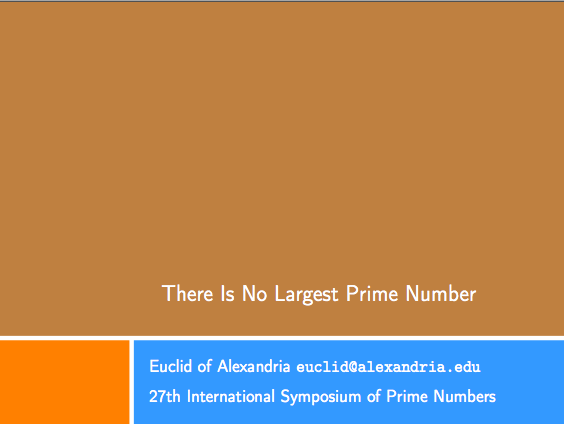
\includegraphics[width=.5\textwidth]{images/Beamer/custom-title-slide}
	\caption{Aspect de la slide de titre du template}
	\label{fig:beamer-custom-title-slide}
\end{figure}

Nous pouvons alors regarder le cas des slides du corps de la présentation.

\subsubsection{Slide générique}
\subParagraphe{Aspect du titre des slides}Ceci se fait via un template appelé \texttt{frametitle}. Ce dernier doit être précisé dans le fichier \texttt{beamerouterthemetexsx.sty}, par exemple :

\begin{lstlisting}[language={[LaTeX]TeX}]
\mode<presentation>

% Frame title
\defbeamertemplate*{frametitle}{texsx}[1][]
{
	\vskip1cm%
	  \begin{beamercolorbox}[wd=\paperwidth,ht=1.2cm]{frametitle} 
		    \begin{tikzpicture}
			      \useasboundingbox[fill=white](0,0) rectangle(\the\paperwidth,1.2);
			        \fill[orange] (0,0) rectangle(2.95,1.2);
				  \fill[blue!50!cyan!80] (3.05,0) rectangle(\the\paperwidth,1.2);
				     \ifx\insertframesubtitle\@empty%
				           {\node[anchor=west, white,font=\large] at (3.2,0.61){\insertframetitle};}
					         \else%
						       {\node[anchor= west, white,font=\large] at (3.2,0.81){\insertframetitle};%
						              \node[anchor= west, white,font=\small] at (3.2,0.41){\insertframesubtitle};}%
							            \fi
								      \end{tikzpicture}
								        \end{beamercolorbox}
									}

									\mode<all>
\end{lstlisting}

Pour faire simple, on exploite le même concept que pour \texttt{titlepage} pour dessiner quelques boîtes, puis on vérifie s'il y a ou non un sous-titre. On définit alors la position du titre et du sous-titre en fonction de cette réponse. Le tout est géré avec des n\oe uds TikZ.

\subParagraphe{Divers éléments}Dans le document d'exemple proposé, on remarque la présence de listes. Ces dernières peuvent être paramétrées avec la commande :

\begin{lstlisting}[language={[LaTeX]TeX}]
\setbeamercolor*{item}{fg=orange}
\end{lstlisting}

Cette commande est à ajouter au fichier \texttt{beamercolorthemetexsx.sty}. On ajoute également la définition des formes des items dans le fichier \texttt{beamerinnerthemetexsx.sty} :

\begin{lstlisting}[language={[LaTeX]TeX}]
% Items
\setbeamertemplate{items}[square]
\setbeamertemplate{sections/subsections in toc}[square]
\end{lstlisting}

Il n'est pas obligatoire que ces déclarations soient dans ce fichier, ceci semble cependant être une norme dans la communauté qui a développé les principaux thèmes Beamer.

On peut alors compiler l'intégralité de la présentation avec notre thème. Des modifications et améliorations peuvent être apportées au thème, qui sont laissées au lecteur intéressé de le faire.



%
% 3 - Ajout table des matières et liste des figures ; tables
%     Utilisation des préférence utilisateurs :
%          * \whereTOC -> end
%          * \whereLOF -> end
%          * \whereLOT -> end
%          * \TOCLOFTNumStyle -> via le fichier de conf xxx
%     Un réglage manuel comlémentaire est possible sur les \vfill - \newpage
%

\setcounter{page}{1}
\renewcommand*{\thepage}{\Roman{page}}

\makeatletter
\ifnum\pdf@strcmp{\whereTOC}{end}=0
\clearpage
\else\ifnum\pdf@strcmp{\whereLOT}{end}=0
\clearpage
\else\ifnum\pdf@strcmp{\whereLOF}{end}=0
\clearpage
\fi\fi\fi

\renewcommand{\sectionbreak}{}
\includeTOC{end}
\includeLOF{end}
\includeLOT{end}

\end{document}


%%% Local Variables:
%%% mode: latex
%%% TeX-master: t
%%% End:
